% SPI modultest

%tekst

I det følgende testes SPI kommunikationen. Alle kommandoer testes for sig og dokumenteres herunder ved oscilloskop billeder samt tabeller der er udarbejdet af eksportedere text filer fra Salae Logic \footnote{Salae Logic er softwaren der benyttes til USB logic analyser. Det er herfra at oscilloskop biller samt data til tabellerne er fra}. 


% Aktiver
\textbf{Aktiver}

Aktiver kommandoen testes vha. testprogrammet ved kommandoen: 


\begin{figure}[h]
\centering
{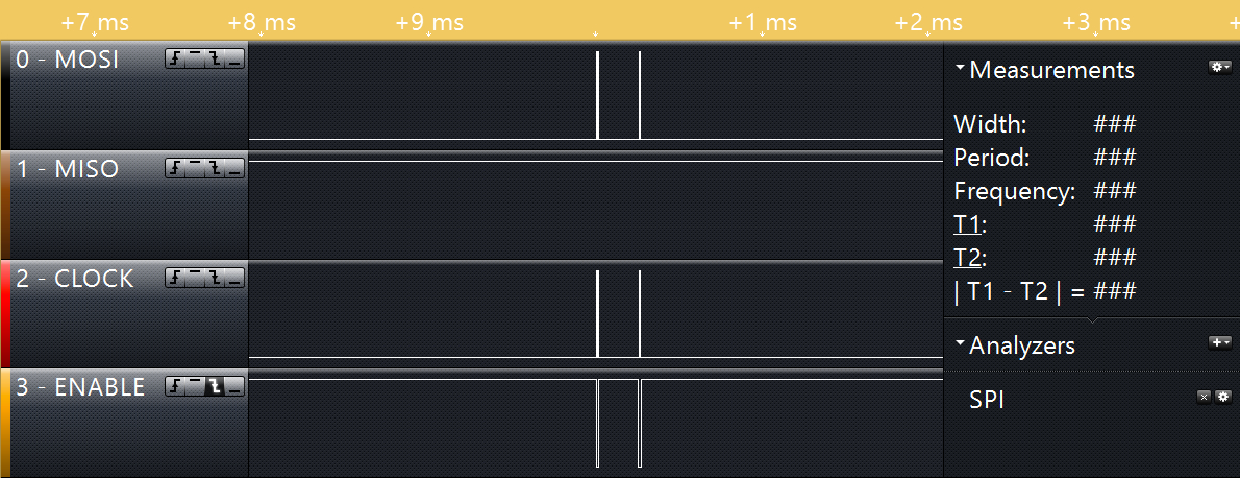
\includegraphics[width=0.90\textwidth]{filer/modultest/Billeder/activate}}
\caption{Oscilloskop billede for kommandoen aktiver}
\label{lab:scop_activate}
\end{figure}

Figur \ref{table:scop_activate} viser dataoverførelsen. Som det ses har kun MOSI betydning for aktiver, da aktiver er en write metode. 

\begin{table}[h]
	\caption{Oscilloskop data eksporteret til tabel}
	\centering
	\begin{tabular}{|l|c|c|}
		\hline 
		\textbf{Char nr} & \textbf{0} & \textbf{1} \\ 		
		\hline 
		\textbf{MOSI} & '\verb+A+' & '\verb+C+' \\ 
		\hline 
		\textbf{MISO} & '\verb+255+' & '\verb+255+' \\ 
		\hline 
	\end{tabular} 
	\label{table:scop_activate}
\end{table}


% Deaktiver
\textbf{Deaktiver}
Deaktiver kommandoen testes vha. testprogrammet ved kommandoen: 


\begin{figure}[h]
\centering
{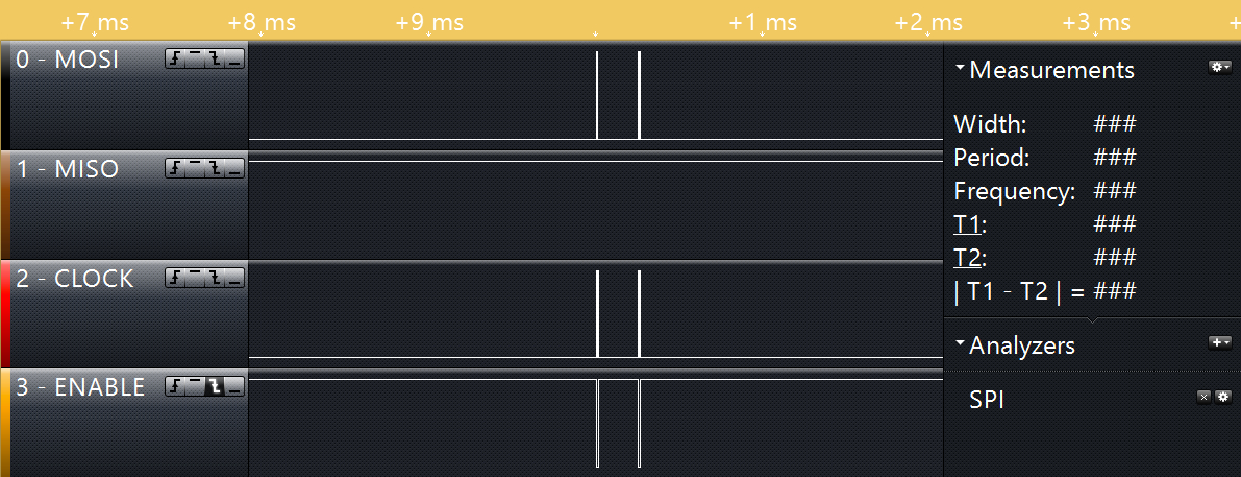
\includegraphics[width=0.90\textwidth]{filer/modultest/Billeder/deactivate}}
\caption{Oscilloskop billede for kommandoen deaktiver}
\label{lab:scop_deactivate}
\end{figure}

Figur \ref{table:scop_deactivate} viser dataoverførelsen. Som det ses har kun MOSI betydning for deaktiver, da deaktiver er en write metode. 

\begin{table}[h]
	\caption{Oscilloskop data eksporteret til tabel}
	\centering
	\begin{tabular}{|l|c|c|}
		\hline 
		\textbf{Char nr} & \textbf{0} & \textbf{1} \\ 		
		\hline 
		\textbf{MOSI} & '\verb+D+' & '\verb+C+' \\ 
		\hline 
		\textbf{MISO} & '\verb+255+' & '\verb+255+' \\ 
		\hline 
	\end{tabular} 
	\label{table:scop_deactivate}
\end{table}


% Deaktiver
\textbf{Config}
Config kommandoen testes vha. testprogrammet ved kommandoen: 


\begin{figure}[h]
\centering
{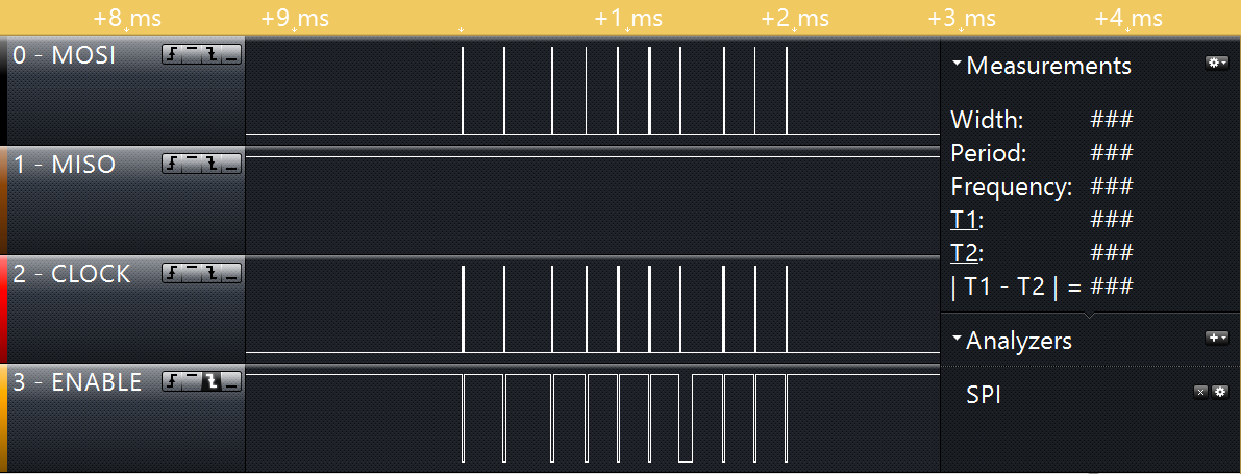
\includegraphics[width=0.90\textwidth]{filer/modultest/Billeder/config}}
\caption{Oscilloskop billede for kommandoen config}
\label{lab:scop_config}
\end{figure}

Figur \ref{table:scop_config} viser dataoverførelsen. Som det ses har kun MOSI betydning for config, da config er en write metode. 

\begin{table}[h]
	\caption{Oscilloskop data eksporteret til tabel}
	\centering
	\begin{tabular}{|l|c|c|c|c|c|c|c|c|c|c|}
		\hline 
		\textbf{Char nr} & \textbf{0} & \textbf{1} & \textbf{2} & \textbf{3} & \textbf{4} & \textbf{5} 
						 & \textbf{6} & \textbf{7} & \textbf{8} & \textbf{9}\\ 		
		\hline 
		\textbf{MOSI} & '\verb+P+' & '\verb+1+' & '\verb+0+' & '\verb+0+' & '\verb+.+' & '\verb+1+' 
						& '\verb+0+' & '\verb+4+' & '\verb+8+' & '\verb+C+' \\ 
		\hline 
		\textbf{MISO} & '\verb+255+' & '\verb+255+' & '\verb+255+' & '\verb+255+' & '\verb+255+' & '\verb+255+' 
						& '\verb+255+' & '\verb+255+' & '\verb+255+' & '\verb+255+' \\ 
		\hline 
	\end{tabular} 
	\label{table:scop_deactivate}
\end{table}


% Verificer
\textbf{Verificer}
Verificer kommandoen testes vha. testprogrammet ved kommandoen: 


\begin{figure}[h]
\centering
{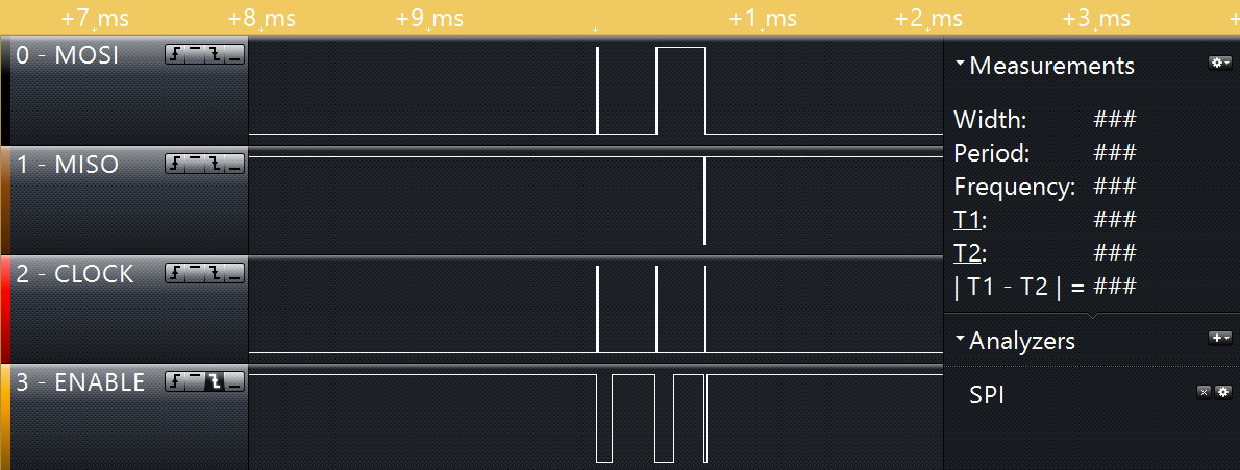
\includegraphics[width=0.90\textwidth]{filer/modultest/Billeder/verify}}
\caption{Oscilloskop billede for kommandoen verificer}
\label{lab:scop_verify}
\end{figure}

Figur \ref{table:scop_verify} viser dataoverførelsen. Som det ses overføres der data på både MOSI og MISO linjen. Det sker da verificer er en read metode. Testen her er udført med tilkoblet Enhed. Hvis enheden kobles fra retuneres ikke ét '1' men derimod '???' 
 

\begin{table}[h]
	\caption{Oscilloskop data eksporteret til tabel}
	\centering
	\begin{tabular}{|l|c|c|c|}
		\hline 
		\textbf{Char nr} & \textbf{0} & \textbf{1} & \textbf{2}\\ 		
		\hline 
		\textbf{MOSI} & '\verb+V+' & '\verb+R+'  & '\verb+C+'\\ 
		\hline 
		\textbf{MISO} & '\verb+255+' & '\verb+255+' & '\verb+1+' \\ 
		\hline 
	\end{tabular} 
	\label{table:scop_verifify}
\end{table}


